%% DONE
\id{ҒТАМР 27.35.33, 76.29.30}{}

\begin{articleheader}
\sectionwithauthors{Н.П.Сапарходжаев, А.А. Умарова, К.Йылмаз, А.А. Умаров, П.И. Сапарходжаев}{ЭКГ СИГНАЛЫНЫҢ ҚАРАПАЙЫМ МОДЕЛІ}

{\bfseries
\textsuperscript{1}Н.П. Сапарходжаев\authorid,
\textsuperscript{2}А.А. Умарова\authorid,
\textsuperscript{3}К. Йылмаз\authorid,
\textsuperscript{1}А.А. Умаров\textsuperscript{\envelope } \authorid,
\textsuperscript{4}П.И. Сапарходжаев\authorid}
\end{articleheader}

\begin{affiliation}
\emph{\textsuperscript{1}Рудный индустриярық университеті, Рудный қ., Қазақстан,}

\emph{\textsuperscript{2}7-ші қалалық клиникалық аурухана, Алматы қ., Қазақстан,}

\emph{\textsuperscript{3}Аднан Мендерес университеті, Айдын қ., Түркия,}

\emph{\textsuperscript{4} Қорқыт Ата атындағы Қызылорда университеті, Қызылорда қ., Қазақстан,}

\raggedright \textsuperscript{\envelope }{\em Корреспондент-автор: e-mail: \href{mailto:uaa_77@mail.ru}{\nolinkurl{uaa\_77@mail.ru}}}
\end{affiliation}

Әлемнің бес континентіндегі 21 елде жүргізілген зерттеулерге сәйкес,
жүрек (жүрек-қан тамырлары) аурулары бүкіл әлемде өлімнің ең көп тараған
себебі болып табылады. Осы себепті жүректі үнемі бақылау және ықтимал
проблемаларды ерте анықтау адам денсаулығы үшін өте маңызды.

Бұл жұмыста қарапайым ЭКГ сигналын модельдеу әдісі ұсынылған.

Жүректің дұрыс жұмыс істеуін анықтау үшін бүкіл әлемде кеңінен
қолданылатын диагностиканың негізгі әдісі - электркардиограмма сигналын
(ЭКГ) өңдеу. Ұсынылған модель пациенттің ЭКГ сигналының маңызды
сегменттерімен жақсы үйлеседі. Бұл жағдайды жүрек проблемаларын оңай
диагностикалау үшін қолдануға болады.

Жұмыстың маңыздылығы - ұсынылған модель PhysioNet дерекқорынан алынған
нақты ЭКГ сигналдарымен салыстырмалы талдау жасау және талдау. Модельдеу
процесінде туындайтын қиындықтар - модель параметрлері әр адам үшін әр
түрлі болады, сонымен бірге олар жасына байланысты бір адам үшін әр
түрлі болады. Нәтижесінде, 20 түрлі ЭКГ жазбалары үшін барлық
сигналдардың алғашқы сегменттері бір - біріне өте жақсы сәйкес келді, ал
қалған бөліктері олардың кезеңдеріндегі айырмашылыққа байланысты сәйкес
келмеді. Сондықтан әр пациентке ЭКГ параметрлерін жеке реттеу қажет.
Орын алған жағдай ЭКГ сигналының бейсызықтығына, жартылай периодты
сипатына байланысты. Бұл мәселені шешу үшін неғұрлым күрделі әдістерді
қолдану қажет.

Дегенмен, ұсынылған модельдің қарапайымдылығы оның қолдану аясын
кеңейтеді және графикалық интерпретацияны жеңілдетеді. Модельді
медициналық мамандықтардың оқу процесінде де қолдануға болады.

{\bfseries Түйін сөздер}: жүрек, сигнал, электркардиограмма (ЭКГ),
математикалық модель, Гаусс функциясы, PhysioNet.

\begin{articleheader}
{\bfseries ПРОСТАЯ МОДЕЛЬ СИГНАЛА ЭКГ}

{\bfseries
\textsuperscript{1}Н.П. Сапарходжаев,
\textsuperscript{2}А.А. Умарова,
\textsuperscript{3}К. Йылмаз,
\textsuperscript{1}А.А. Умаров\textsuperscript{\envelope },
\textsuperscript{4}П.И. Сапарходжаев}
\end{articleheader}

\begin{affiliation}
\emph{\textsuperscript{1}Рудненский индустриальный университет, г. Рудный, Казахстан,}

\emph{\textsuperscript{2}7-ая городская клиническая больница, г. Алматы, Казахстан,}

\emph{\textsuperscript{3}Университет Аднана Мендереса, г. Айдын, Турция,}

\emph{\textsuperscript{4}Кызылординский университет имени Коркыт Ата, г. Кызылорда, Казахстан,}

\emph{e-mail: \href{mailto:uaa_77@mail.ru}{\nolinkurl{uaa\_77@mail.ru}}}
\end{affiliation}

Согласно исследованиям, проведенным в 21 стране на пяти континентах
мира, сердечные (сердечно-сосудистые) заболевания являются наиболее
частой причиной смерти во всем мире. По этой причине регулярный
мониторинг сердца и раннее выявление потенциальных проблем имеют
решающее значение для здоровья человека.

Цель работы заключается в предложенном простом методе моделирования
сигнала ЭКГ.

Основным методом диагностики, широко используемым во всем мире для
определения правильного функционирования сердца, является обработка
сигнала электрокардиограммы (ЭКГ). Представленная модель хорошо
сочетается с важными сегментами сигнала ЭКГ пациента в спокойном
состояний. Это состояние можно использовать для легкой диагностики
проблем с сердцем.

Важность работы состоит в том, что представленная модель сравнивается и
анализируется с реальными сигналами ЭКГ, полученными из базы данных
PhysioNet. Трудности, возникающие в процессе моделирования, заключаются
в том, что параметры модели будут отличными для каждого человека, и в то
же время, они в зависимости от возраста будут различными для одного и
того же человека. В результате для 20 различных записей ЭКГ первые
сегменты всех сигналов идеально совпадали друг с другом, а остальные
части не совпадали друг с другом из-за разницы в их периодах. Поэтому
каждому пациенту требуется индивидуальная настройка параметров ЭКГ.
Такая ситуация обусловлена нелинейностью - то есть полупериодным
характером сигнала ЭКГ. Для решения этой проблемы необходимо
использовать более сложные методы.

Однако простота предлагаемой модели расширяет область ее применения и
упрощает графическую интерпретацию. Модель может быть также использована
в учебном процессе медицинских специальностей.

{\bfseries Ключевые слова:} сердце, сигнал, электрокардиограмма (ЭКГ),
математическая модель, Функция Гаусса, PhysioNet.

\begin{articleheader}
{\bfseries SIMPLE ECG SIGNAL MODEL}

{\bfseries
\textsuperscript{1}N.P. Saparkhojayev,
\textsuperscript{2}A.A. Umarova,
\textsuperscript{3}K. Yilmaz,
\textsuperscript{1}A.A. Umarov\textsuperscript{\envelope },
\textsuperscript{4}P.I. Saparkhojayev}
\end{articleheader}

\begin{affiliation}
\emph{\textsuperscript{1}Rudny industrial university, Rudny, Kazakhstan,}

\emph{\textsuperscript{2}7th City Clinical Hospital, Almaty, Kazakhstan,}

\emph{\textsuperscript{3}Adnan Menderes University, Aydin, Turkey,}

\emph{\textsuperscript{4} Korkyt Ata Kyzylorda University, Kyzylorda, Kazakhstan}

\emph{e-mail: \href{mailto:uaa_77@mail.ru}{\nolinkurl{uaa\_77@mail.ru}}}
\end{affiliation}

According to studies conducted in 21 countries on five continents of the
world, heart (cardiovascular) diseases are the most common cause of
death worldwide. For this reason, regular heart monitoring and early
detection of potential problems are crucial for human health.

The purpose of the work is to propose a simple method for modeling the
ECG signal.

The main diagnostic method widely used worldwide to determine the proper
functioning of the heart is electrocardiogram (ECG) signal processing.
The presented model fits well with important segments of the
patient' s ECG signal in a calm state. This condition can
be used to easily diagnose heart problems.

The importance of the work lies in the fact that the presented model is
compared and analyzed with real ECG signals obtained from the PhysioNet
database. The difficulties that arise in the modeling process are that
the model parameters will be different for each person, and at the same
time, they will be different for the same person depending on age. As a
result, for 20 different ECG recordings, the first segments of all the
signals perfectly matched each other, and the remaining parts did not
match each other due to the difference in their periods. Therefore, each
patient needs to individually adjust the ECG parameters. This situation
is due to non-linearity - that is, the semi-periodic nature of the ECG
signal. To solve this problem, it is necessary to use more sophisticated
methods.

However, the simplicity of the proposed model expands the scope of its
application and simplifies graphical interpretation. The model can also
be used in the educational process of medical specialties.

{\bfseries Keywords:} heart, signal, electrocardiogram (ECG), mathematical
model, Gauss function, PhysioNet.

\begin{multicols}{2}
{\bfseries Кіріспе.} Жүрек - барлық тіршілік иелері үшін өмірлік маңызы бар
ағза мүшесі. Егер жүрек дұрыс жұмыс істемесе, ол денсаулыққа елеулі
проблемаларды тудырады, тіпті өлімге әкелуі мүмкін. Бес континенттің 21
елінде жүргізілген зерттеулерге сәйкес {[}1{]}, жүрекке байланысты
(жүрек-қан тамырлары) аурулар дүние жүзінде өлімнің ең көп тараған
себебі болып табылады. Осы себепті жүректі үнемі бақылау және ықтимал
проблемаларды ерте анықтау адам денсаулығы үшін өте маңызды.

Жүректің дұрыс жұмыс істеп тұрғанын анықтау үшін бүкіл әлемде кеңінен
қолданылатын ең негізгі сигнал -- электркардиограмма (ЭКГ) сигналы. Бұл
сигналдар біздің әлемдегі ең танымал электрлік сигналдардың бірі болып
табылады. Көптеген адамдар бұл сигналдардың жүрекпен және біздің
денсаулығымызбен тығыз байланысты екенін біледі, алайда бұл сигналдың
пішінін дұрыс елестете алмайды. ЭКГ сигналдары негізінен жүректің
электрлік белсенділігін білдіреді және олар 1-суретте көрсетілгендей
типтік формаға ие.
\end{multicols}

\begin{figure}[H]
	\centering
	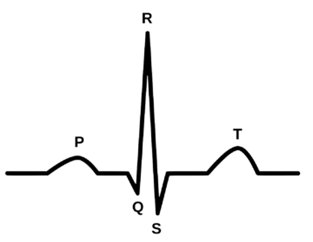
\includegraphics[width=0.4\textwidth]{media/ict/image40}
	\caption*{1 - сурет. ЭКГ сигналының пішіні {[}2{]}}
\end{figure}

\begin{multicols}{2}
ЭКГ сигналы жүректің электрлік белсенділігінің нәтижесі болып табылады
және әрбір сау адамда ұқсас болады. Бұл сигнал формасындағы әдеттен тыс
ауытқулар (бұрмалану) жүректегі ықтимал проблемаларды көрсетеді.
Дәрігерлер 70 жылдан астам уақыт бойы аритмия және миокард инфарктісі
сияқты жүрек ауруларын анықтау үшін ЭКГ сигналдарын қолданып келеді.
Әдеттегі ЭКГ сигналы 1-суретте көрсетілгендей P, Q, R, S және T
толқындарынан тұрады {[}2{]}. Жүрек ауруларын диагностикалау үшін әр
бөліктің пішіні мен уақыт аралықтары және әр түрлі тістер арасындағы
қашықтық қолданылады {[}2{]}. Жүректің және сәйкес ЭКГ сигналының
байланысы 2-суретте көрсетілген {[}3{]}.
\end{multicols}

\begin{figure}[H]
	\centering
	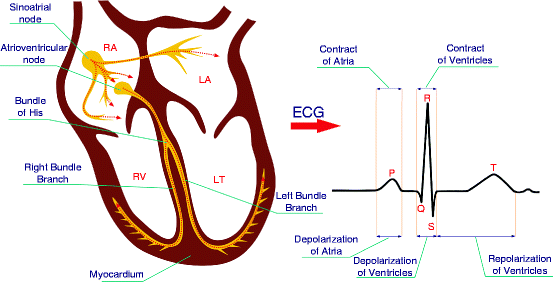
\includegraphics[width=0.75\textwidth]{media/ict/image41}
	\caption*{2 - сурет. Жүрек және ЭКГ сигнал арасындағы байланыс}
\end{figure}

\begin{multicols}{2}
ЭКГ сигналын түсіру құрылғылары өте қарапайым, арзан және қауіпсіз
жүйелер, сондықтан олар бүкіл әлемде кеңінен қолданылады. Дегенмен,
артефактілер (байқаусыз қимылдар) мен шу деп аталатын көптеген факторлар
ЭКГ сигналдарының кездейсоқ секірулерін тудыруы мүмкін. Бұл артефактілер
пациенттердің қозғалысы, науқасқа электродтың қозғалысы және
электромагниттік кедергілер болуы мүмкін. Сондықтан таза және тұрақты
ЭКГ сигналын алу үшін осы артефактілер мен шуды ЭКГ сигналдарынан алып
тастау керек. ЭКГ сигналдарын жақсарту үшін толқын пішінін түрлендіру
сияқты әртүрлі әдістер қолданылады. Толығырақ ақпаратты {[}4-9{]}
сайтынан табуға болады.

ЭКГ сигналдарын талдаудан басқа, осы сигналдарды модельдеу бойынша
зерттеулер әдебиеттерде де кең орын алады {[}10-18{]}. ЭКГ сигналдарын
модельдеу арқылы жүректі электрлік түсіну және мүмкін болатын жүрек
ауруларын анықтау әлдеқайда жеңіл және жылдамырақ болуы мүмкін. Бұл
мақалада ЭКГ сигналдары Гаусс тәрізді сигналдардың комбинациясы арқылы
қарапайым түрде модельденетін болады.

Біздің ұсынылып отырған модель 1-суреттегі ЭКГ сигналының типтік
моделіне негізделген және нақты ЭКГ сигналдары "PhysioNet" сайтынан
алынып, пайдаланылады {[}19,20{]}.

{\bfseries Материалдар мен әдістер.} \emph{ЭКГ сигналдары.} Әдеттегі ЭКГ
сигналы 1-суретте көрсетілгендей белгілі пішінге ие. Осы суреттен көріп
отырғанымыздай, әдеттегі ЭКГ сигналында 3 негізгі компонент бар. Олар
``тістер'' деп те аталады. Бұл P толқыны, QRS күрделі толқыны және T
толқыны деп аталады. U толқыны деп аталатын төртінші компонент ЭКГ
сигналына енгізілгенімен, көптеген модельдерде бұл компонент еленбейді.
ЭКГ сигналының типтік моделін, оның ішінде U толқынын 3-суреттен көруге
болады.
\end{multicols}

\begin{figure}[H]
	\centering
	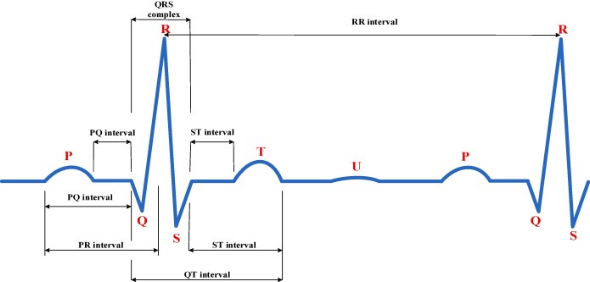
\includegraphics[width=0.8\textwidth]{media/ict/image42}
	\caption*{3 - сурет. U толқынын қосықандағы ЭКГ моделі}
\end{figure}

\begin{multicols}{2}
U толқындары ЭКГ сигналдарында жиі байқалмайды. Екінші жағынан, әдеттегі
ЭКГ сигналына P, Q, R, S және T бөліктері кіреді. Сондықтан бұл
зерттеуде U толқыны қарастырылмады және жұмыстың негізінде 1-суретте
келтірілген ЭКГ сигналы алынды.

Кез-келген адамның әдеттегі ЭКГ сигналы -- 1-суретте берілген сигналдың
мерзімді кеңеюі болып табылып, 3-суретті береді. Сондықтан бұл сигналдың
периодын анықтау оны модельдеу үшін өте маңызды. Сол сияқты, әрбір
толқынның (P, QRS және T) орналасуы, сондай-ақ олардың ені мен
амплитудасы да маңызды болады. Тағы бір маңыздысы, бұл параметрлер
адамнан адамға және мезгіл-мезгіл бір адам үшін де өзгеріп отырады. Бұл
жағдай Physionet дерекқорынан алынған нақты ЭКГ сигналының көмегімен
түсіндіріледі {[}18-20{]}.

4-суретте {[}20{]} ЭКГ сигналын көруге болады. Осы мәліметтер базасының
және жазылған ЭКГ сигналдарының егжей-тегжейлері келесі бөлімде
айтылады.

Зерттеуде ерекшелігі - ЭКГ сигналының жиілігі тұрақты емес болғаны. ЭКГ
сигналы периодты деп есептелсе де, ол периодты емес, өйткені тізбекті Q
шыңдар арасындағы қашықтық тұрақты емес. 4-суретте. 4, тізбекті r
шыңдарының арақашықтықтары сәйкесінше 0.750 с, 0.814 с, 0.932 с және
0.934 с құрайды. Сол сияқты, әрбір r шыңының шамасы әр PQRST
интервалында әр түрлі болады. Демес, ЭКГ сигналын периодты емес,
жартылай периодты деп санауға болады. Нәтижесінде бір PQRST
интервалындағы ЭКГ сигналын модельдеу бірінші PQRST толқынымен сәйкес
келеді, бірақ оның жартылай периодтық сипатына байланысты басқа PQRST
толқындарымен кейбір қателер болады.
\end{multicols}

\begin{figure}[H]
    \centering
    \begin{subfigure}{0.49\textwidth}
        \centering
        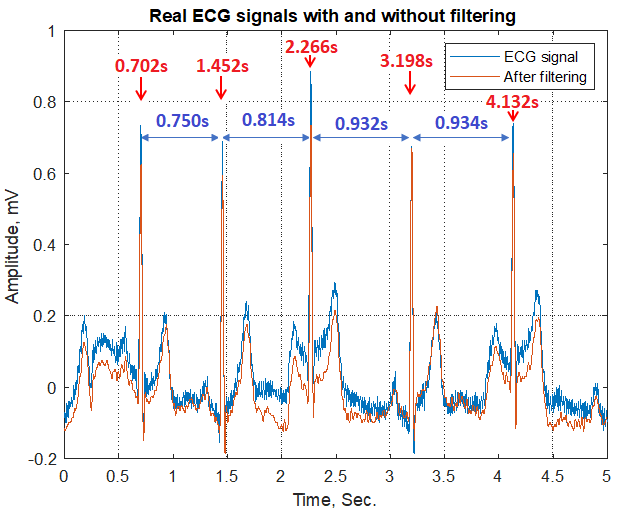
\includegraphics[width=\linewidth]{media/ict/image43}
        \caption*{4 - сурет. Physionet дерекқорынан алынған ЭКГ\vspace{4mm}}
    \end{subfigure}
    \hfill
    \begin{subfigure}{0.49\textwidth}
        \centering
        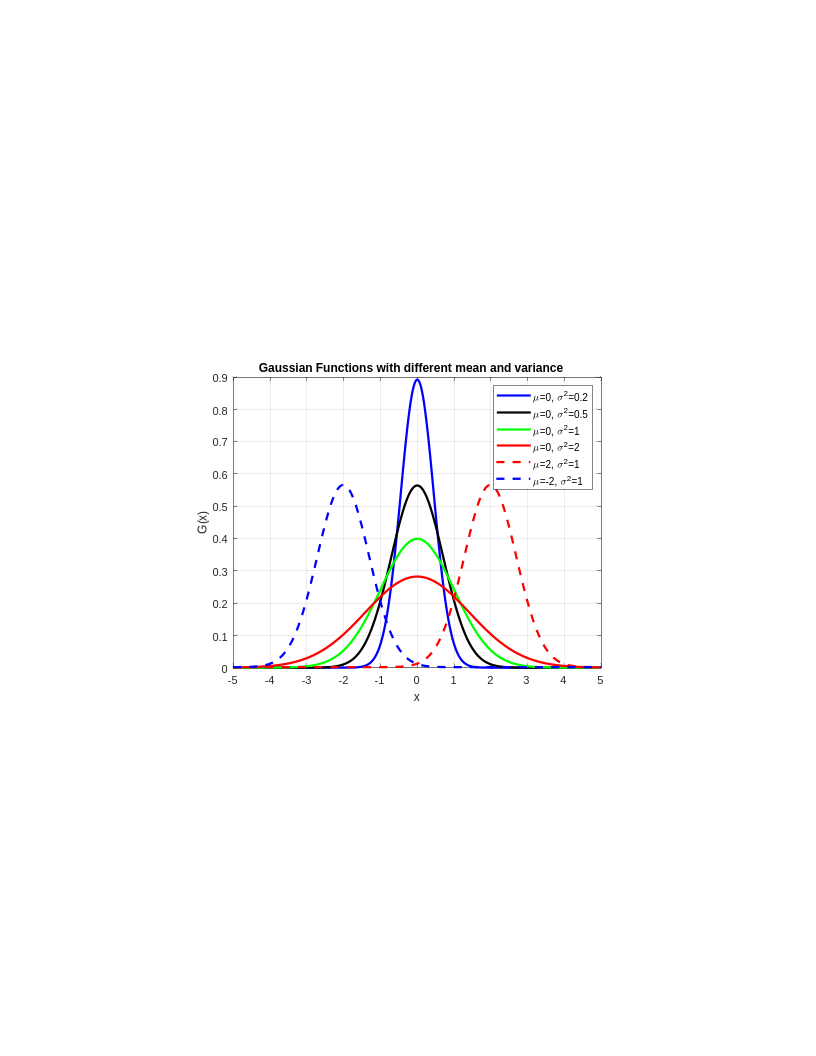
\includegraphics[width=\linewidth]{media/ict/image44}
        \caption*{5 - сурет. Гаусс функциялары және әртүрлі дисперсия мәндері}
    \end{subfigure}
\end{figure}

\begin{equation}
    G(x) = \frac{A}{\sqrt{2\pi\sigma^{2}}}\exp\left( - \frac{(x - \mu)^{2}}{2\sigma^{2}} \right)
\end{equation}

\begin{multicols}{2}
ЭКГ сигналын модельдеудің ең оңай жолы - P, QRS тістерін және T
толқындарына бөлек сәйкес келетін симметриялы "қоңырау қисығы"
сипаттамалары берілген Гаусс функциясы ретінде пайдалану. Гаусс
функциялары ықтималдық тығыздығы функциясын қалыпты түрде бөлінген
кездейсоқ айнымалы (x) функциясын μ математикалық күтім (немесе орташа),
σ дисперсия және A амплитуда мәнімен өрнектеледі {[}19{]}.

\emph{Гаусс функциясы арқылы ЭКГ сигналын модельдеу.} 1-суретте
көрсетілгендей, әдеттегі ЭКГ сигналына Гаусс функцияларына ұқсас P, R
және T шыңдары кіреді. Демек, ЭКГ сигналдарын Гаусс функцияларымен
моделдеу орынды. PhysioNet сайтынан Гаусс функциялары үшін қажетті
параметрлерді алуға болады.

MIT Есептеу Физиологиясы Зертханасының мүшелері басқаратын PhysioNet
физиологиялық және клиникалық деректердің үлкен жинақтарына және соған
байланысты ашық бастапқы бағдарламалық жасақтамаға тегін қол жеткізуді
қамтамасыз етеді {[}19, 20{]}. Бұл платформада көптеген биомедициналық
сигналдарды алуға және қолдануға болады.
\end{multicols}

\begin{figure}[H]
	\centering
	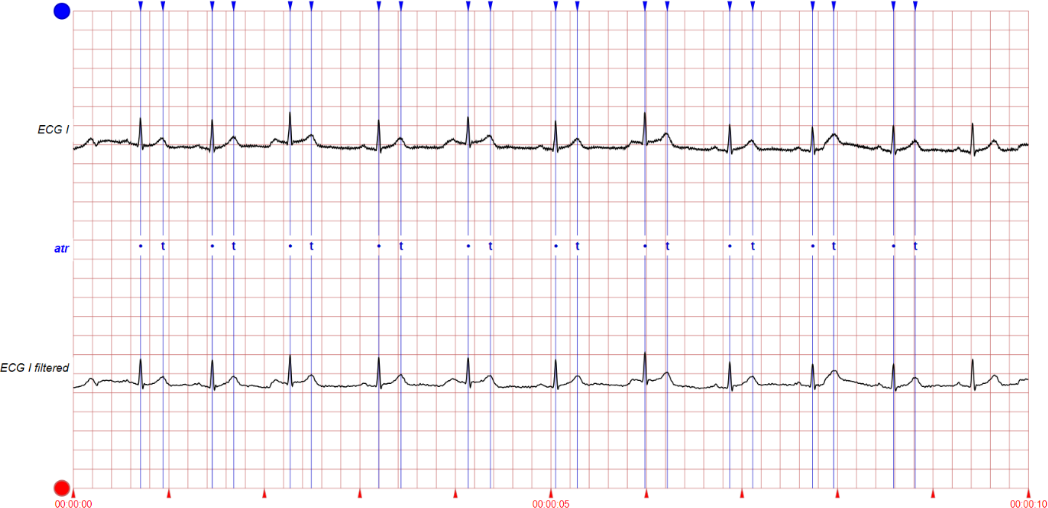
\includegraphics[width=\textwidth]{media/ict/image45}
	\caption*{6 - сурет. PhysioNet дерекқорынан (Person\_01/rec\_1) түрінде алынған ЭКГ сигналдардың пішіні}
\end{figure}

\begin{figure}[H]
    \centering
    \begin{subfigure}{0.50\textwidth}
        \centering
        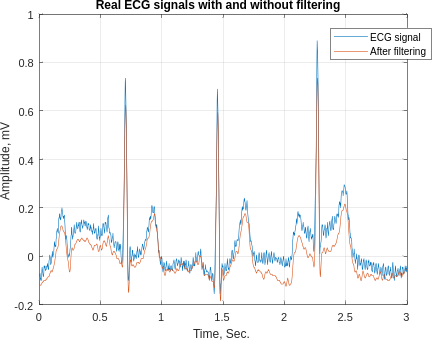
\includegraphics[width=\linewidth]{media/ict/image46}
        \caption*{Person\_01/rec\_1}
    \end{subfigure}
    \hfill
    \begin{subfigure}{0.475\textwidth}
        \centering
        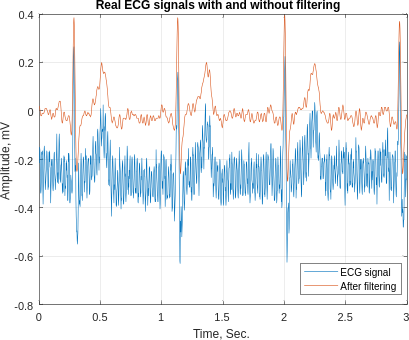
\includegraphics[width=\linewidth]{media/ict/image47}
        \caption*{Person\_02/rec\_1}
    \end{subfigure}
    \caption*{7 - сурет. PhysioNet сайтынан 2 түрлі адам үшін алынған ЭКГ сигналды MATLAB ортасында қайта түрлендіру}
\end{figure}

\begin{multicols}{2}
Осы мақалада ECG-ID дерекқоры қолданылады. ECG-ID дерекқоры - Татьяна
Луговая өз магистрлік диссертациясында жинап қолданған және Физиобанк
үшін құрбан еткен 90 еріктілердің (волонтер) 310 ЭКГ жиынтығы {[}20{]}.
ЭКГ сигналдары 20 секунд ішінде жазылады, 12 битпен 500 Гц жиілікте
цифрланады. Жазбалар еріктілерден алынды (автордың студенттері,
әріптестері және достары болған 13 пен 75 жас аралығындағы 44 ер адам
мен 46 әйел). Әр адамға арналған жазбалар саны 2-ден (бір күн ішінде
жиналған) 20-ға дейін (6 ай ішінде мезгіл-мезгіл жиналған) өзгереді.
Өңделмеген шикі ЭКГ сигналдары өте шулы және жоғары және төмен жиілікті
шуды қамтиды. Әрбір жазба шикі және сүзілген сигналдарды қамтиды.
Жазылған ЭКГ сигналдарын PhysioNet платформасының
``\href{https://physionet.org/lightwave/?db=ecgiddb/1.0.0}{Visualize
waveforms}'' құралының көмегімен 6-суреттегідей көруге болады. Біздің
еңбекте осы деректер MATLAB ортасында өңделіп, пайдаланылады (7-сурет).

\emph{ЭКГ сигналының моделі.} Ұсынылған әдісте ЭКГ сигналының P, Q, R, S
және T сегменттері Гаусс функцияларын қолдана отырып жеке-жеке
модельденеді. Сондықтан әрбір бөліктің орташасын және дисперсиясын
анықтау керек. Сонымен қатар, әрбір сегменттің шамалары мен ЭКГ
сигналының периоды да анықталуы керек. 4-суретте көрсетілгендей, PQRST
толқыны жартылай периодты сипатта болады. 4-суретте адамның ЭКГ сигналы
көрсетілген, сол сияқты әр түрлі адам үшін әр түрлі жиіліктегі ЭКГ
сигналдары болуы тиіс. Бұл жағдайды 8-суреттен анық көруге болады -
әртүрлі адамдардың ЭКГ сигналдары әртүрлі. Барлық сигналдар бірінші P
сегменттері қабаттасатын етіп ауыстырылады. Алғашқы Р сегменттері
қабаттасқанымен, келесі Р сегменттері әр түрлі уақытта жүреді, бұл әрбір
жазыған ЭКГ сигналының әр түрлі кезеңдері бар екенін көрсетеді. Мұнда
Person\_01 (Person\_01/rec\_1, rec\_2, rec\_3, rec\_4, rec\_5) 5 жазбасы
қолданылады {[}19{]}.

4,7 және 8-суреттерден көріп отырғанымыздай, ЭКГ сигналдарының
сипаттамалары ұқсас, алайда, қайта сканерленген соң шамалы
айырмашылықтары бар екені айқын. Сондықтан олардың кез келгенін
анықтамалық сигнал ретінде таңдау керек.
\end{multicols}

\begin{figure}[H]
	\centering
	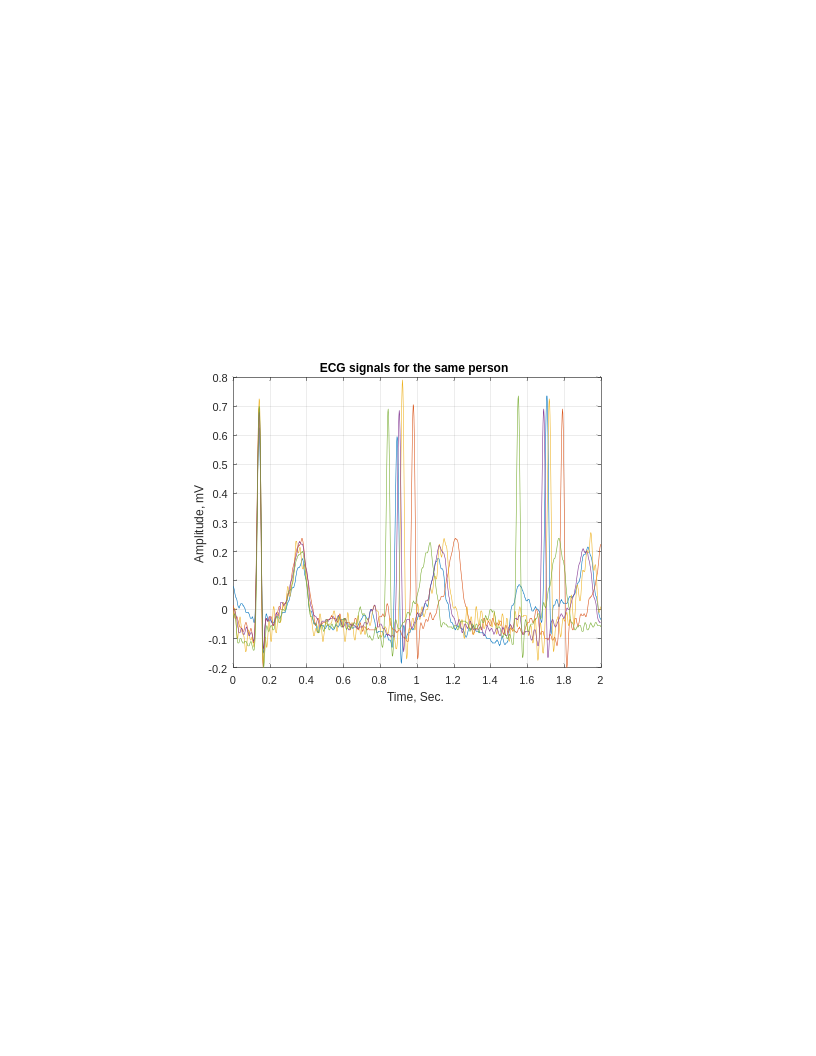
\includegraphics[width=0.6\textwidth]{media/ict/image48}
	\caption*{8-сурет. Бір адамның әр түрлі мезгілдегі сүзгіленген ЭКГ (Person\_01/rec\_1, rec\_2, rec\_3, rec\_4, rec\_5 data))}
\end{figure}

\begin{multicols}{2}
P, Q, R, S және T сегменттері (1) көмегімен 1-кестедегі параметрлері
арқылы модельденеді. PhysioNet жазбаларында ЭКГ сигналдары 500 Гц
жиілікте цифрланған 20 секунд ішінде жазылады, яғни әрбір ЭКГ деректері
секундына 500 үлгіні қамтиды. Ұсынылған модельде сигнал аралығы 2 секунд
болып таңдалады. Сөйтіп, барлығы 1000 үлгіні құрайды. Осы 1000 үлгі (2
секунд) ЭКГ сигналының бір кезеңіне сәйкес келеді. Жоғарыда айтылғандай,
ЭКГ сигналдарының периоды тұрақты емес. ЭКГ сигналдарын талдау арқылы
сигналдың периоды эксперименталды түрде 800 мс болып таңдалады, бұл 400
үлгіге сәйкес келеді. Яғни, 1000 үлгідегі ЭКГ моделі 400 үлгіні
түрлендірді. 9-суретте алынған p, Q, R, S, T сегменттерін және жалпы ЭКГ
сигналын көруге болады.
\end{multicols}

{\bfseries 1-кесте. Ұсынылған модельдегі Гаусс функция параметрлері}
\begin{table}[H]
\centering
\begin{tblr}{
  cells = {c},
  hlines,
  vlines,
}
\textbf{Модель параметрлері} & \textbf{P} & \textbf{Q} & \textbf{R} & \textbf{S} & \textbf{T}\\
\textbf{µ} & 0.08 & 0.224 & 0.234 & 0.264 & 0.460\\
{\bfseries $\sigma$\textsuperscript{2}} & 0.001 & 0.012 & 0.008 & 0.005 & 0.001\\
\textbf{A} & 0.008 & -0.0105 & 1 & 0.2 & 0.015
\end{tblr}
\end{table}

\begin{figure}[H]
	\centering
	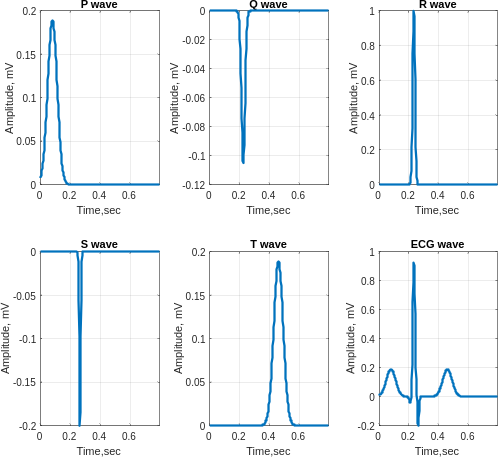
\includegraphics[width=0.8\textwidth]{media/ict/image49}
	\caption*{9-сурет. P, Q, R, S, T сегменттер және толық 1 периодты ЭКГ сигналы}
\end{figure}

\begin{multicols}{2}
{\bfseries Нәтижелер мен талқылау}. {\bfseries Нәтижелерді талқылау.} Бұл
бөлімде ұсынылған модель PhysioNet дерекқорынан алынған нақты ЭКГ
сигналдарымен салыстырылады {[}19{]}.

2-бөлімде көрсетілгендей, PhysioNet-те ЭКГ сигналдары екі түрде
беріледі: бастапқы ЭКГ сигналдары және сүзілген ЭКГ сигналдары. Мұнда
ұсынылған әдіспен салыстыру үшін сүзілген ЭКГ сигналдары қолданылады.
10-суретте ұсынылған модель 1, 4-ші адам жазбаларының сүзілген ЭКГ
сигналдарымен салыстырылады. Көріп отырғанымыздай, сигналдардың шығу
тегі әр жазба үшін әр түрлі, сондықтан сигналдарды қабаттасу үшін баптау
(калибрлеу) керек. Бірінші R шыңының орнын сигналдарды қабаттастыру үшін
пайдалануға болады. Осы себепті MATLAB-та бірінші R шыңы анықталады және
сигналдардың барлық R шыңдары қабаттасады. Нәтиже 11-суретте 1-ші
адамның 20 түрлі ЭКГ жазбалары үшін көрсетілген. Көріп отырғанымыздай,
барлық сигналдардың бірінші сегменттері бір-біріне өте жақсы сәйкес
келеді, екінші жағынан, олардың кезеңдерінің айырмашылығына байланысты
қалған бөліктерді бір-біріне жабыстыру мүмкін болмады. 12-суретте
ұсынылған ЭКГ моделі көрсетілген.
\end{multicols}

\begin{figure}[H]
	\centering
	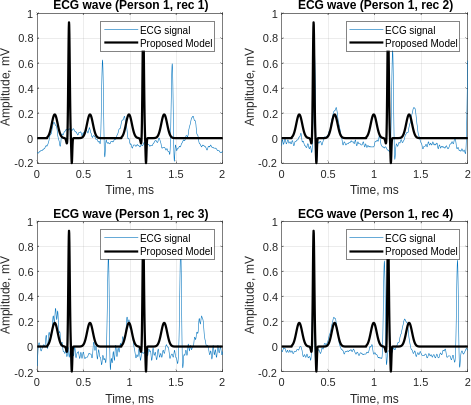
\includegraphics[width=0.7\textwidth]{media/ict/image50}
	\caption*{10 - сурет. Ұсынылған модель мен дәл ЭКГ сигналдарын салыстыру (1-ші адам)}
\end{figure}

\begin{figure}[H]
	\centering
	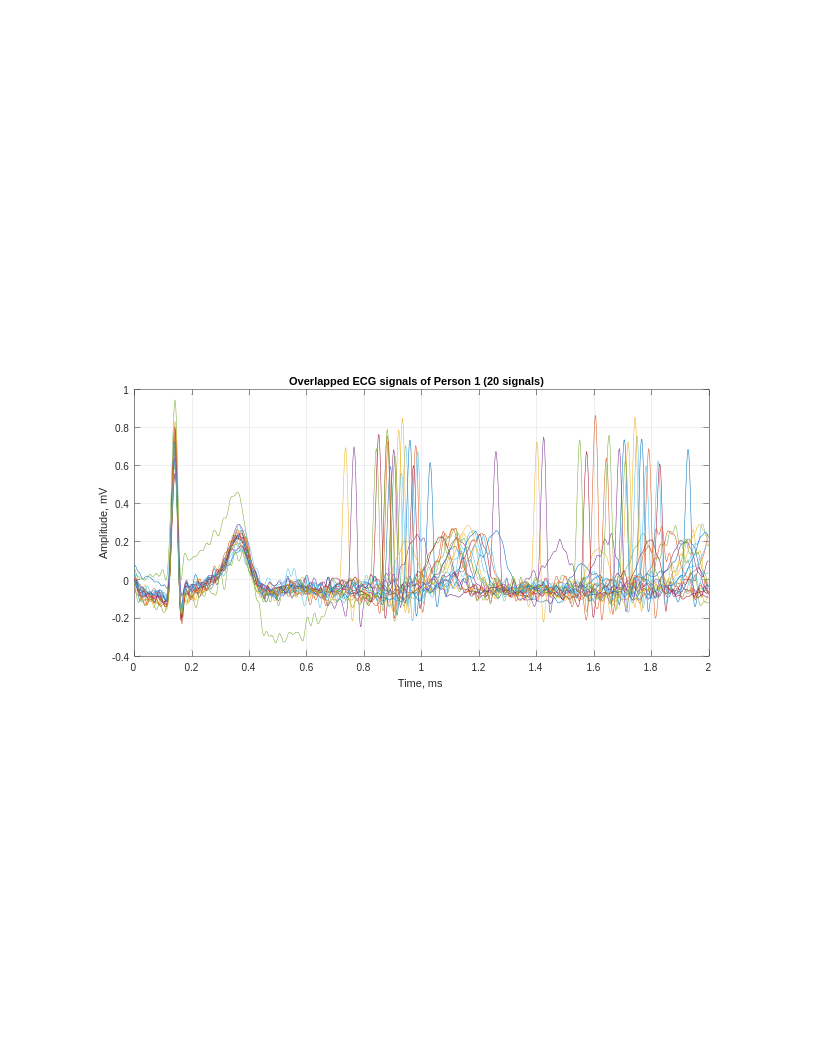
\includegraphics[width=0.8\textwidth]{media/ict/image51}
	\caption*{11 - сурет. Әрбір сигналдың бірінші R шыңдарын пайдаланатын қабаттасқан ЭКГ сигналдары (1, 20-шы адам жазбалары)}
\end{figure}

\begin{figure}[H]
	\centering
	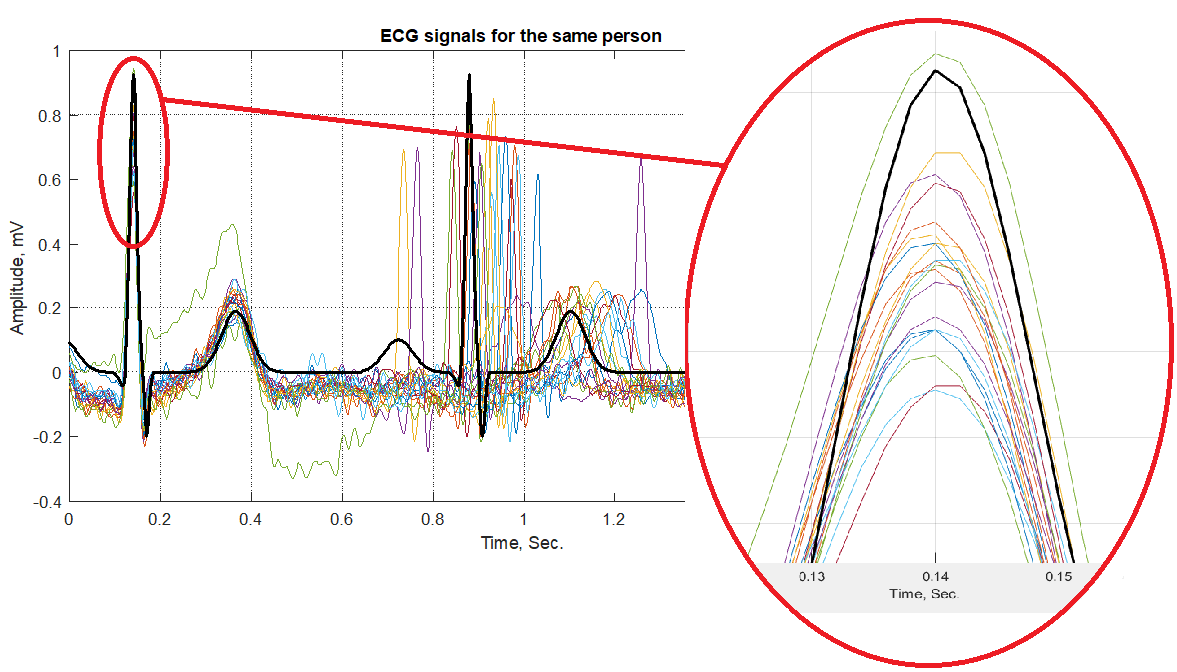
\includegraphics[width=0.8\textwidth]{media/ict/image52}
	\caption*{12 - сурет. Ұсынылған модель және қабаттасқан ЭКГ сигналдары (1, 20-шы адам жазбалары). Қара сигнал ұсынылған модельді білдіреді}
\end{figure}

\begin{figure}[H]
	\centering
	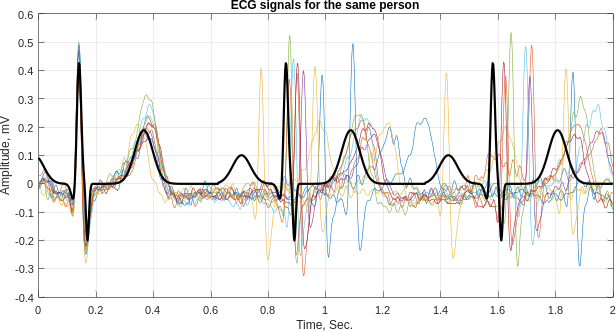
\includegraphics[width=0.8\textwidth]{media/ict/image53}
	\caption*{13 - сурет. Ұсынылған модель және қабаттасқан ЭКГ сигналдары (2, 10-шы адам жазбалары). Қара сигнал ұсынылған модельді білдіреді}
\end{figure}

\begin{multicols}{2}
{\bfseries Қорытынды.} Осы мақалада дәл ЭКГ сигналдарын талдау арқылы ЭКГ
сигналының қарапайым моделі ұсынылған. Ұсынылған модельде ЭКГ сигналының
әр түрлі сегменттері үшін орташа, дисперсиялық және амплитудалық
параметрлері әр түрлі Гаусс функциялары қолданылады. PhysioNet дерекқоры
нақты ЭКГ сигналдарын алу үшін пайдаланылады және модельдеу нәтижелері
осы сигналдармен салыстырылады.

Ұсынылған модель науқастың тыныш қарапайым жағдайдағы ЭКГ сигналының
маңызды сегменттерімен жақсы үйлеседі. Бұл жағдай жүрек проблемаларын
оңай диагностикалау үшін қолданылуы мүмкін. ЭКГ сигналының жартылай
периодтық сипаты модельдеудің негізгі мәселесі болып табылады. Бұл
мәселе күрделі әдістерді қолдану арқылы шешілуі мүмкін. Аталған мәселені
біз болашақ еңбектерімізде қарастырамыз. Сонымен қатар, аритмия және
миокард инфарктісі сияқты жүрек-қан тамырлары аурулары мен ЭКГ
сигналдарын модельдеу - жұмыстың тағы бір болашақ бағыты болып табылады.
\end{multicols}

\begin{center}
{\bfseries Әдебиеттер}
\end{center}

\begin{references}
1. Dagenais, G. R.~et al.~Variations in common diseases, hospital
admissions, and deaths in middle-aged adults in 21 countries from five
continents (PURE): A prospective cohort study// The~Lancet.- 2020.-
Vol.395(10226).-P.785-794 DOI 10.1016/S0140-6736(19)32007-0.

2. Aziz, S., Ahmed, S. \& Alouini, MS. ECG-based machine-learning
algorithms for heartbeat \\classification//~Sci Rep.-2021.-Vol11(1):18738/
\href{https://doi.org/10.1038/s41598-021-97118-5}{DOI
10.1038/s41598-021-97118-5}.

3. Gacek, A. (2011). An Introduction to ECG Signal Processing and
Analysis. In: Gacek, A., Pedrycz, W. (eds) ECG Signal Processing,
Classification and Interpretation. Springer, London.
\href{https://doi.org/10.1007/978-0-85729-868-3_2}{DOI
10.1007/978-0-85729-868-3\_2}

4. Clifford, G. D., Azuaje, F. \& McSharry, P. Advanced methods and
tools for ECG data analysis
//\href{https://www.researchgate.net/journal/BioMedical-Engineering-OnLine-1475-925X?_tp=eyJjb250ZXh0Ijp7ImZpcnN0UGFnZSI6InB1YmxpY2F0aW9uIiwicGFnZSI6InB1YmxpY2F0aW9uIn19}\\{BioMedical
Engineering OnLine}Artech. -2006.-Vol.6(1).- P.1-3. DOI
\href{http://dx.doi.org/10.1186/1475-925X-6-18}{10.1186/1475-925X-6-18}

5. Malmivuo, J. \& Plonsey, R. Bioelectromagnetism: Principles and
Applications of Bioelectric and \\Biomagnetic fields~(Oxford University
Press, 1995). - 512 p. ISBN 9780195058239

6. Moody, G. B. \& Mark, R. G. The impact of the MIT-BIH arrhythmia
database.~IEEE Eng. Med. Biol. Mag.- 2001.- Vol.~20(3).- P.45--50 DOI
\href{https://doi.org/10.1109/51.932724}{10.1109/51.932724}

7. Thiamchoo, N. \& Phukpattaranont, P. Application of wavelet transform
and shannon energy on R peak detection algorithm. In~International
Conference on Electrical Engineering/Electronics, Computer,
Telecommunications and Information Technology (ECTI-CON). P. 1--5
(2016).

DOI 10.1109/ECTICON.2016.7561280

8. Mabrouki, R., Khaddoumi, B. \& Sayadi, M. R peak detection in
electrocardiogram signal based on a combination between empirical mode
decomposition and Hilbert transform. In~IEEE International \\Conference on
Advanced Technologies for Signal and Image Processing (ATSIP).
P.183--187 (2014). DOI\\
\href{http://dx.doi.org/10.1109\%2FATSIP.2014.6834603}{10.1109/ATSIP.2014.6834603}

9. Elgendi, M. Terma framework for Biomedical signal analysis: An
economic-inspired approach. \\Biosensors.- 2016.- Vol.6(4).- P.55 - 69.
\href{https://doi.org/10.3390/bios6040055}{DOI 10.3390/bios6040055}

10. Awal, Md. Abdul et al. Simplified mathematical model for generating
ecg signal and fitting the model using nonlinear least square technique/
Conference: International Conference on Mechanical Engineering,
2011.-P.1-6

11.
\href{https://www.researchgate.net/scientific-contributions/Pavol-Dolinsky-2111486589?_sg\%5B0\%5D=OpDWPWB7F-xsKNW7QhdA72wrK8fp7beQ04-y1V0k2OSl-vY7yVCBibx1np_IexfBvwzs1tc.3cwJN3iOVCnhElwMBHi_44SzEhdGHYZWVIVDkbQ1O1b7A14CJ6y-CqFfnB303LWj8pCAkU8V0IFoKmFKiUohPw&_sg\%5B1\%5D=AVFGn2hkG-rhmm2v1aXJV9E-zSTVwesxqk3bJDU_jEY7VSRsfP3brCGDMfFzLd-5yvpDVx0.qPkk_lpV-CUBkVH8P4FChkQpEOFV8sRGeKQiTftWsOp6D_liXpE1YL21VpUyx-lJcgXk9ynFK7DYQ-rBYDhYVA}{Dolinský},
P., Andras, I., Michaeli, L., Grimaldi, D. Model for generating simple
synthetic ecg signals//
\href{https://www.researchgate.net/journal/Acta-Electrotechnica-et-Informatica-1338-3957?_tp=eyJjb250ZXh0Ijp7ImZpcnN0UGFnZSI6InB1YmxpY2F0aW9uIiwicGFnZSI6InB1YmxpY2F0aW9uIiwicG9zaXRpb24iOiJwYWdlSGVhZGVyIn19}{Acta
Electrotechnica et Informatica}.- 2018.-Vol.~18(3):3-8. DOI
\href{http://dx.doi.org/10.15546/aeei-2018-0019}{10.15546/aeei-2018-0019}.

12. Awal, M..A., Mostafa, S.S., Ahmad, M., Alahe, M.A.,Rashid, M.A.,
Kouzani, A.Z.;,Mahmud, M.A.P. Design and Optimization of ECG Modeling
for Generating Different Cardiac Dysrhythmias//Sensors.-
2021.-Vol.21(5): 1638. DOI 10.3390/ s21051638.

13. Mukhopadhyay, S., Sircar, P. Parametric modelling of ECG
signal//~Med. Biol. Eng. Comput.-1996.-Vol.~34.- P.171- 174.
\href{https://doi.org/10.1007/BF02520024}{DOI 10.1007/BF02520024}.

14. Mohamed Lamine TALBI, Philippe Ravier. Flexible ECG signal modeling
and compression using alpha stable functions// Medical Engineering \&
Physics.-2022.-Vol.109: 103865

\href{https://doi.org/10.1016/j.medengphy.2022.103865}{DOI
10.1016/j.medengphy.2022.103865}.

15. E. Adib, A. S. Fernandez, F. Afghah and J. J. Prevost .Synthetic ECG
Signal Generation Using \\Probabilistic Diffusion Models. In~IEEE
Access.-2023.- Vol.11.- P. 75818-75828

DOI 10.1109/ACCESS.2023.3296542.

16. Faal, M., \& Almasganj, F. ECG Signal Modeling Using Volatility
Properties: Its Application in Sleep Apnea Syndrome//~Journal of
healthcare engineering.-~2021: 4894501.

\href{https://doi.org/10.1155/2021/4894501}{DOI 10.1155/2021/4894501}.

17. Koski AModelling ECG signals with hidden Markov models //Artificial
intelligence in medicine.-1996.-Vol.~8(5).-P. 453- 471.
\href{https://doi.org/10.1016/S0933-3657(96)00352-1}{DOI
10.1016/S0933-3657(96)00352-1}.

18. Molavi-Arabshahi, M., Jalil, R., \& Yousefi, M. A new mathematical
model for reconstruction ECG signal based on non-polynomial cubic
spline//~Journal of Mathematical Modeling.-2022.-Vol.~10(1).- P.107-117.
DOi10.22124/jmm.2021.18796.1609.

19. PhysioNet -The Research Resource for Complex Physiologic Signals.-
\href{https://physionet.org}{https://physionet.org} - Data obrashhenija 01.08.2024

20. Lugovaja T.S. Biometricheskaja identifikacija cheloveka po
jelektrokardiogramme. {[}Magisterskaja dissertacija{]}
Fakul' tet vychislitel' nyh tehnologij i
informatiki, SPbGJeTU «LJeTI», Sankt-Peterburg, Rossijskaja Federacija;
ijun'{} 2005 g.{[}in Russian{]}
\end{references}

\begin{authorinfo}
\emph{{\bfseries Авторлар туралы мәліметтер:}}

Сапарходжаев~Н.П.~-~PhD,~қауымдастырылған~профессор, Басқарма
Төрағасы~-- Ректор, «Рудный индустриялық университеті» КЕАҚ, Рудный қ.,
Қазақстан,
e-mail:\href{mailto:nursp81@gmail.com}{\nolinkurl{nursp81@gmail.com}};

Умаров А. А.- PhD, доцент м.а., «Рудный индустриялық университеті» КЕАҚ,
Рудный қаласы, Қазақстан, e-mail:\\
\href{mailto:uaa_77@mail.ru}{\nolinkurl{uaa\_77@mail.ru}};

Умарова А.А.- Кардиология мамандығы бойынша резидент, Алматы қаласындағы
7-қалалық клиникалық ауруханасының кардиолог-дәрігері, Алматы қаласы,
Қазақстан, e-mail:
\href{mailto:amankelgikyzy15@gmail.com}{\nolinkurl{amankelgikyzy15@gmail.com}};

Йылмаз Калкан - PhD, профессор, Аднан Мендерес атындағы Университет,
Айдын қаласы, Түркия, e-mail:\\
\href{mailto:yilmaz.kalkan@adu.edu.tr}{\nolinkurl{yilmaz.kalkan@adu.edu.tr}};

Сапарходжаев П. И.-педагогика ғылымдарының кандидаты,Коркыт Ата атындағы
Кызылорда университетінің профессоры Қызылорда қ. Қазақстан,
pajarbek\_52@mail.ru

\emph{{\bfseries Information about the authors}}

Saparkhojayev N. P.-PhD, Associate Professor, Chairman of the Board --
Rector, NLC "Rudny Industrial University", Rudny, Kazakhstan, e-mail:
\href{mailto:nursp81@gmail.com}{\nolinkurl{nursp81@gmail.com}};

Umarov А.А.- PhD, Acting Associate Professor, NLC "Rudny Industrial
University", Rudny, Kazakhstan, e-mail: \\uaa\_77@mail.ru;

Umarova А.А.-Resident in Cardiology, Cardiologist at the 7th City
Clinical Hospital in Almaty, Almaty, Kazakhstan, e-mail:
amankelgikyzy15@gmail.com;

Yilmaz Kalkan -PhD, Professor, Adnan Menderes University, Aydın, Turkey,
e-mail: yilmaz.kalkan@adu.edu.tr;

Saparkhojayev P. I.-Candidate of Pedagogical Sciences, Professor at
Korkyt Ata Kyzylorda University, Kyzylorda, Kazakhstan, e-mail:
\href{mailto:pajarbek_52@mail.ru}{\nolinkurl{pajarbek\_52@mail.ru}}.
\end{authorinfo}
